
%%%%%%%%%%%%%%%%%%%%%%%%%%%%%%%%%%%%%%%%%%%%%%%%%%%%%%%%%%%%%%%%%%%%%%%%%%%%%%%%%%%%%%%
\section{Deep Learning}
\label{section:deep_learning}
%%%%%%%%%%%%%%%%%%%%%%%%%%%%%%%%%%%%%%%%%%%%%%%%%%%%%%%%%%%%%%%%%%%%%%%%%%%%%%%%%%%%%%%

Broadly speaking, machine learning is a field of engineering using data to improve on a task at hand \cite{Goodfellow-et-al-2016}. A subfield of machine learning called deep learning uses multi-layer \acp{ANN} for the improvement process. 

An \ac{ANN} is a model whose goal is to approximate some function $f^*$ \cite{Goodfellow-et-al-2016}. A \emph{feedforward network} or an \ac{MLP} is an input-to-output mapping. For example, in the context of audio signal processing, $f^*$ could be a mapping of an input signal $s_{in}(t)$ to an output signal $s_{out}(t)$, i.\ e., $s_{out}(t) = f^*(s_{in}(t))$. The mapping $f$ defined by an \ac{MLP}, $\hat{s}_{out}(t) = f(s_{in}(t); \pmb{\theta})$, is dependent on the parameter vector $\pmb{\theta}$. The learning process aims at finding a parameter vector $\pmb{\theta^*}$ that allows for a sufficiently accurate approximation of $f^*$ by $f$.

% TODO: Add figure with a MLP

A feedforward network consists of \emph{layers} which define the subsequent stages of computations. The first layer is called the \emph{input layer} and the last layer is called the \emph{output layer}. The layers in between are called the \emph{hidden layers}, because we do not observe their output directly. Each layer consists of a set of \emph{units}: affine transformations of unit's inputs followed by a nonlinearity. Each unit in a layer receives outputs of all units in the previous layer at its input and outputs a single scalar. The number of layers determines the \emph{depth} of the model. Feedforward networks with at least 1 hidden layer are called \emph{deep}. The number of units in a layer determines its \emph{width}.

More formally, the $l$-th layer of an \ac{MLP} outputs a vector $\pmb{y}^{(l)}$ according to the following formula

\begin{equation}
  \pmb{y}^{(l)} = g ( \pmb{W}^{(l)} \pmb{y}^{(l-1)} + \pmb{b}^{(l)}),
  \label{eq:mlp_forward_pass}
\end{equation}
where $\pmb{W}^{(l)}$ is the weight matrix of the $l$-th layer with the $i$-th row associated with the $i$-th unit in the layer, $\pmb{b}$ is a vector of units' biases, $g(\cdot)$ is a nonlinear function applied element wise, and $\pmb{y}^{(0)}$ is the network's input vector. In this notation, $f(\pmb{y}^{(0)};\pmb{\theta}) = \pmb{y}^{(L)}$, where $L$ denotes the number of layers of the \ac{MLP}.

Most common nonlinearity functions are hyperbolic tangens ($\tanh$), \ac{ReLU} (\Equation{eq:relu}), and the logistic sigmoid function $\sigma$ (\Equation{eq:logistic_sigmoid}) \cite{Goodfellow-et-al-2016}

\begin{align}
  \text{ReLU}(x) &= \max\{0, x\},\label{eq:relu}\\
  \sigma (x) &= \frac{1}{1 + \exp (-x)}.\label{eq:logistic_sigmoid}
\end{align}

\acp{MLP} are \emph{universal function approximators}, i.\ e., they can approximate an arbitrary function (fulfilling very mild criteria) with an arbitrarily small error given enough width or depth \cite{Goodfellow-et-al-2016}.

% TODO: Add a note on the notation used to describe MLPs

%%%%%%%%%%%%%%%%%%%%%%%%%%%%%%%%%%%%%%%%%%%%%%%%%%%%%%%%%%%%%%%%%%%%%%%%%%%%%%%%%%%%%%%
\section*{Architectures}
%%%%%%%%%%%%%%%%%%%%%%%%%%%%%%%%%%%%%%%%%%%%%%%%%%%%%%%%%%%%%%%%%%%%%%%%%%%%%%%%%%%%%%%

As deep learning is a widely and actively pursued field of science, there exist many different neural network architectures beyond the \ac{MLP}. They are often designed for the task at hand using expert knowledge or heuristics \cite{Goodfellow-et-al-2016}. In this section, two highly successful architectures are presented, both of them relevant for this thesis.

%%%%%%%%%%%%%%%%%%%%%%%%%%%%%%%%%%%%%%%%%%%%%%%%%%%%%%%%%%%%%%%%%%%%%%%%%%%%%%%%%%%%%%%
\subsection*{Long Short-Term Memory}
%%%%%%%%%%%%%%%%%%%%%%%%%%%%%%%%%%%%%%%%%%%%%%%%%%%%%%%%%%%%%%%%%%%%%%%%%%%%%%%%%%%%%%%

\Ac{RNN} is a neural network that maintains a \emph{feedback} connection, i.\ e., a connection from its output to its input. Typically, to calculate the current output, the previous output is taken as part of the input. This step-by-step processing is characteristic to sequence modeling, where \acp{RNN} are found most useful.

A particularly successful \ac{RNN} architecture is the \ac{LSTM} \cite{Hochreiter1997}. \ac{LSTM} uses \emph{gating units} to allow or disallow its \emph{memory cells} to be updated during processing. This helps to learn long-term dependencies which are crucial for the network to maintain a notion of a context.

A memory cell $i$ has an associated state vector at time step $t$ denoted $\pmb{c}_t$. The output of a memory cell is the \emph{hidden state} $\pmb{h}_t$, which is an element-wise (Hadamard) product of the output gate $\pmb{o}_t$ and the cell state processed by hyperbolic tangent

\begin{equation}
  \pmb{h}_t = \pmb{o}_t \odot \tanh (\pmb{c}_t).
  \label{eq:lstm_hidden_state}
\end{equation}

Output gate's purpose is to determine whether the cell will produce output at time step $t$. Output gate is a function of the current input and the previous hidden state

\begin{equation}
  \pmb{o}_t = \sigma (\pmb{W}_{io} \pmb{x}_t + \pmb{b}_{io} + \pmb{W}_{ho} \pmb{h}_{t-1} + \pmb{b}_{ho}),
  \label{eq:lstm_output_gate}
\end{equation}

where $\pmb{x}_t$ is the cell's input at time $t$, $\pmb{W}_{io}$ and $\pmb{W}_{ho}$ are output gate's weight matrices for input and hidden state respectively, $\pmb{b}_{io}$ and $\pmb{b}_{ho}$ are the output gate's bias vectors, and $\sigma$ denotes the sigmoid function (\Equation{eq:logistic_sigmoid}) applied element-wise.

Input gate vector $\pmb{i}_t$ and forget gate vector $\pmb{f}_t$ are defined analogously

\begin{align}
  \pmb{i}_t &= \sigma (\pmb{W}_{ii} \pmb{x}_t + \pmb{b}_{ii} + \pmb{W}_{hi} \pmb{h}_{t-1} + \pmb{b}_{hi}), \label{eq:lstm_input_gate}\\
  \pmb{f}_t &= \sigma (\pmb{W}_{if} \pmb{x}_t + \pmb{b}_{if} + \pmb{W}_{hf} \pmb{h}_{t-1} + \pmb{b}_{hf}). \label{eq:lstm_forget_gate}
\end{align}

The input gate determines the amount of information introduced to the cell state from the current input. The forget gate controls the amount of information preserved from the previous cell state. Finally, at each time step, the cell state is updated as follows

\begin{equation}
  \pmb{c}_t = \pmb{f}_t \odot \pmb{c}_{t-1} + \pmb{i}_t \odot \pmb{g}_t,
  \label{eq:lstm_cell_update}
\end{equation}

where $\pmb{g}_t$ represents the proposed update to the cell state

\begin{equation}
  \pmb{g}_t = \tanh (\pmb{W}_{ig} \pmb{x}_t + \pmb{b}_{ig} + \pmb{W}_{hg} \pmb{h}_{t-1} + \pmb{b}_{hg}),
  \label{eq:lstm_proposed_update}
\end{equation}

which has its own weight matrices $\pmb{W}_{ig}, \pmb{W}_{hg}$, and bias vectors $\pmb{b}_{ig}, \pmb{b}_{hg}$.

In order of computations, at time step $t$, we calculate the values of the gating vectors $\pmb{i}_t, \pmb{f}_t, \pmb{o}_t$ (\Equationst{eq:lstm_input_gate}{eq:lstm_forget_gate}{eq:lstm_output_gate} respectively), the proposed cell state update (\Equation{eq:lstm_proposed_update}), update the cell state (\Equation{eq:lstm_cell_update}), and the hidden state, which is also the output (\Equation{eq:lstm_hidden_state}) \cite{Pytorch}. The computational dependencies are depicted in \Figure{fig:lstm_memory_cell}.

\begin{figure}
  \centering
  \def\svgwidth{\columnwidth}
  \input{figures/svg/lstm.pdf_tex}
  \caption{Computational graph of a single time step of an \ac{LSTM} cell. Empty cells mark placeholders for intermediate calculations.}
  \label{fig:lstm_memory_cell}
\end{figure}

\ac{LSTM} cells can be stacked in layers. The input to the $l$-th layer is the output of the $(l-1)$-th layer, $\pmb{x}_t^{(l)} = \pmb{h}_y^{(l-1)}$, with $\pmb{x}_t^{(0)} = \pmb{x}_t$ being the network input at time $t$.

% TODO: Add a note that Alec used an MLP on the LSTM's output

In audio processing, \ac{LSTM} has been successfully applied to guitar amplifier modeling \cite{Wright2019,Wrightetal2020} and time-varying effects modeling \cite{Wright2020}.

%%%%%%%%%%%%%%%%%%%%%%%%%%%%%%%%%%%%%%%%%%%%%%%%%%%%%%%%%%%%%%%%%%%%%%%%%%%%%%%%%%%%%%%
\subsection*{Residual Networks}
%%%%%%%%%%%%%%%%%%%%%%%%%%%%%%%%%%%%%%%%%%%%%%%%%%%%%%%%%%%%%%%%%%%%%%%%%%%%%%%%%%%%%%%

\begin{figure}
  \centering
  \begin{tikzpicture}
    \node[dspnodeopen,dsp/label=above]              (x) {$\pmb{x}$};
    \node[dspnodefull, right=of x]              (c0) {};
    \node[coordinate,above=of c0] (c1) {};
    \node[dspsquare,right=of c1] (network) {$h(\pmb{x})$};
    \node[coordinate,right=of network] (c3) {};
    \node[dspadder,below=of c3,yshift=1mm] (adder) {};
    \node[dspnodeopen,right=of adder,dsp/label=above] (fx) {$f(\pmb{x})$};

    \draw[dspline] (x) -- (c0);
    \draw[dspline] (c0) -- (c1);
    \draw[dspconn] (c1) -- (network);
    \draw[dspline] (network) -- (c3);
    \draw[dspconn] (c3) -- (adder);
    \draw[dspconn] (c0) -- (adder);
    \draw[dspconn] (adder) -- (fx);
\end{tikzpicture}

  \caption{A residual block (ResBlock). $h(\pmb{x})$ represents the network learning the residual and $f(\pmb{x})$ represents the network's output.}
\end{figure}

Another architecture significant to this work is the \ac{ResNet} \cite{He2015}. Its characteristic feature is the so-called \emph{\ac{ResBlock}} containing a \emph{skip connection}. The skip connection provides a direct path from the input to the output which allows for summing the input with the network's output. It effectively makes the network learn not the mapping $f^*(\pmb{x})$ but the residual $h^*(\pmb{x}) = f^*(\pmb{x}) - \pmb{x}$. On the one hand, it alleviates the problem of the \emph{vanishing gradient} \cite{Goodfellow-et-al-2016} and eventually allows for training very deep architectures with hundreds of layers \cite{He2015}. Depth is one of the most significant factors in neural network design, thus, being able to train deeper and deeper architectures allows for improving performance on the desired tasks. On the other hand, the skip connection can simplify the training process; instead of learning a complete function, the network must only learn its residual. For example, if the true mapping is the identity function, it is easier to learn the residual (which is $0$ everywhere) rather than the identity itself, which would involve approximating a hyperplane with nonlinear units \cite{He2015}.

%%%%%%%%%%%%%%%%%%%%%%%%%%%%%%%%%%%%%%%%%%%%%%%%%%%%%%%%%%%%%%%%%%%%%%%%%%%%%%%%%%%%%%%
\subsection*{State Trajectory Network}
%%%%%%%%%%%%%%%%%%%%%%%%%%%%%%%%%%%%%%%%%%%%%%%%%%%%%%%%%%%%%%%%%%%%%%%%%%%%%%%%%%%%%%%

A \ac{ResNet}-based architecture that was successfully applied to \ac{VA} modeling is the \acf{STN} \cite{Parker2019}. In this approach, a schematic of the electronic circuit of the device under study is analyzed and the voltage value across the capacitors is combined to form the state vector of a state-space description. The goal is to learn the state transitions and the relation between the state and the output. To facilitate this task, not the full mapping is learned by the network but just the residual (the \emph{trajectory} of the state). One of the elements of the state is associated with the output sample. The whole state is supplied together with current input sample as the input used to compute the next state, therefore, rendering the network recurrent. Gathering data to determine the true state requires voltage measurements inside the modeled device. 


\begin{figure}
  \centering
  \scalebox{0.7}{\input{figures/svg/stn.pdf_tex}}
  \caption{\Acf{STN} architecture. After \cite{Parker2019}.}
  \label{fig:stn}
\end{figure}

The architecture of \ac{STN} is shown in \Figure{fig:stn}. The layers $l_1, \dots, l_L$ are fully-connected and, thus, form an \ac{MLP}. A novelty in \ac{STN} in comparison to \ac{ResNet} is the presence of the residual scaling factor $h_\tau$. In \cite{Parker2019}, it is defined as

\begin{equation}
  h_\tau = \frac{f_{s\text{, train}}}{f_{s\text{, processing}}},
\end{equation}
where $f_{s\text{, train}}, f_{s\text{, processing}}$ are the sampling rates used at train time and at processing time respectively. According to the authors, if the sampling rate at processing time is higher than the one used at training, high-frequency behavior of the original system may be lacking. Using sampling rates at processing time lower than the one used at training (without any additional antialiasing facility) can result in aliasing behavior. The aliasing aspect is important to this work and \ac{STN} naturally fits as a model to compare the tested methodology to.

As most the recurrent architectures, \ac{STN} can be trained using teacher forcing as explained in \Section{subsec:teacher_forcing}.
% TODO: Check the number of this section.

%%%%%%%%%%%%%%%%%%%%%%%%%%%%%%%%%%%%%%%%%%%%%%%%%%%%%%%%%%%%%%%%%%%%%%%%%%%%%%%%%%%%%%%
\subsection*{Residual Integration Network, Bilinear Block}
%%%%%%%%%%%%%%%%%%%%%%%%%%%%%%%%%%%%%%%%%%%%%%%%%%%%%%%%%%%%%%%%%%%%%%%%%%%%%%%%%%%%%%%

The introduction of the \ac{ResNet} raised interest in its interpretation as an Euler step of solving differential equations \cite{Chen2018}.
This led to several architectures whose parametrization is similar to the popular numerical schemes of solving \acp{ODE}.

One of such architectures is the \acf{RINN} \cite{Ouala2019}.
In this approach, the residual is computed using $S$ stages of computations, each calculating one part of the residual. The neural network used for each stage is shared among the stages. The outputs of the stages are summed with weights which may either correspond to a numerical scheme or may be learned jointly with the neural network parameters.

\Ac{RINN} using the \ac{RK} scheme of order 4 is depicted in \Figure{fig:rinn4}. The coefficients $\alpha_{\_}$ and $\beta_{\_}$ may be fixed according to \Table{tab:rk4_tableau} or learned from data jointly with the parameters of network F.

\begin{figure}
  \centering
  \scalebox{0.83}{\input{figures/svg/rinn4.pdf_tex}}
  \caption{\Acl{RINN} architecture. Each block marked with F is the same neural network. After \cite{Fablet2017}.}
  \label{fig:rinn4}
\end{figure}

\begin{figure}
  \centering
  \scalebox{0.7}{\input{figures/svg/bilinear_block.pdf_tex}}
  \caption{A bilinear block architecture for computing a part of the residual. After \cite{Fablet2017}.}
  \label{fig:bilinear_block}
\end{figure}

The neural network chosen in \cite{Ouala2019}
for the parametrization of each stage consists of three fully-connected layers. The output of the first one is concatenated with the element-wise product of the output of the two remaining layers. The goal of the element-wise multiplication is to enable second-order interactions between the variables. This parametrization is called a \emph{bilinear block} \cite{Fablet2017} and is shown in \Figure{fig:bilinear_block}. $\pmb{x}_t$ denotes the input to the bilinear block at time $t$, layers $l_1, l_2,$ and $l_3$ are fully-connected and $F(t, \pmb{x}_t)$ is the partial residual. If the number of stages $S$ is equal to 1 and time step is equal to 1, then $F(t, \pmb{x}_t)$ is the full residual. The physical interpretation of the bilinear block depends on the computation scheme in which it is used and the modeled problem.



%%%%%%%%%%%%%%%%%%%%%%%%%%%%%%%%%%%%%%%%%%%%%%%%%%%%%%%%%%%%%%%%%%%%%%%%%%%%%%%%%%%%%%%
\section*{Training of Neural Networks}
%%%%%%%%%%%%%%%%%%%%%%%%%%%%%%%%%%%%%%%%%%%%%%%%%%%%%%%%%%%%%%%%%%%%%%%%%%%%%%%%%%%%%%%

Training of \acp{ANN} is done using an optimization algorithm from the \emph{gradient descent} family of algorithms \cite{Goodfellow-et-al-2016}. In general, gradient descent methodology requires specifying a \emph{loss} or a \emph{target function} between the network's output and the desired output. The optimization then proceeds by sampling a \emph{minibatch} of examples from the \emph{training set} in each iteration, processing them with the network, and calculating the loss. The loss function is a measure of dissimilarity (or distance) between the network's output and the \emph{target}. For example, the training set may consist of images (inputs) with associated labels (targets). The network should learn the mapping from an image to its label. After calculating the loss, the gradient of the loss with respect to the network's parameters (mainly weights and biases) is computed via \emph{backpropagation} through the network using the chain rule of derivatives. After calculating the gradient of the loss with respect to each individual parameter, a step in the direction of the negated gradient is performed (steepest descent). The size of the step is determined by the \emph{learning rate}. Some algorithms use a different step size for each parameter, for example, Adam \cite{Kingma2017}.

%%%%%%%%%%%%%%%%%%%%%%%%%%%%%%%%%%%%%%%%%%%%%%%%%%%%%%%%%%%%%%%%%%%%%%%%%%%%%%%%%%%%%%%
\subsection*{Loss Functions}
%%%%%%%%%%%%%%%%%%%%%%%%%%%%%%%%%%%%%%%%%%%%%%%%%%%%%%%%%%%%%%%%%%%%%%%%%%%%%%%%%%%%%%%

In order to train, test, and compare machine learning models, we need a performance measure \cite{Goodfellow-et-al-2016}. For supervised learning problems, i.e., problems where the targets of the training set are known, a natural approach is to measure the error between the network's output and the target values. One of the most popular metrics is the \ac{MSE}

\begin{equation}
  \mathcal{E}_\text{MSE}(y, \hat{y}) = \frac{1}{N} \sum \limits_{n=0}^{N-1} (y[n] - \hat{y}[n])^2,
\end{equation}
where $y$ is the target signal, $\hat{y}$ is the network's output and $N$ is the length of these two signals.

In the context of audio processing, the \ac{MSE} loss has the drawback that it prioritizes errors of signals with large dynamics and neglects the inaccuracies of quiet parts \cite{Parker2019}. These quiet parts are often perceptually relevant. Therefore, a relative error measure is thought to be more suitable in audio applications.

A commonly used relative error measure in \ac{VA} modeling is the \ac{ESR} \cite{Wright2019,Wright2019a, Wrightetal2020,Wright2020}

\begin{equation}
  \mathcal{E}_\text{ESR}(y, \hat{y}) = \frac{\sum_{n=0}^{N-1} (y[n] - \hat{y}[n])^2}{\sum_{n=0}^{N-1} (y[n])^2},
\end{equation}
i.e., the energy of the error signal divided by the energy of the target signal.

In order to suppress the DC offset in the network's output a DC loss term may be added to the loss function \cite{Wright2019a,Wright2020}
\begin{equation}
  \mathcal{E}_\text{DC}(y, \hat{y}) = \frac{\left(\frac{1}{N} \sum_{n=0}^{N-1} (y[n] - \hat{y}[n])\right)^2}{\frac{1}{N} \sum_{n=0}^{N-1} (y[n])^2}.
\end{equation}

Additionally, it is important to take the perceptual aspect into account by penalizing errors that result in less perceptually convincing results. This can be achieved using a \emph{pre-emphasis filter}, i.e., a filter that boosts the perceptually relevant frequencies and suppresses the irrelevant ones.

A first-order highpass filter can be used as a pre-emphasis filter as shown in \cite{Wright2019,Wrightetal2020,Wright2020}. Such a filter has a transfer function of the form

\begin{equation}
  H(z) = 1 - 0.85 z^{-1}.
\end{equation}

This form of pre-emphasis is straightforward to implement, achieves perceptually superior performance to non-preemphasized loss functions, and is just slightly inferior to much more complicated pre-emphasis filters \cite{Wright2019a}.

After \cite{Wright2019a,Wright2020,Wright2019}, this works uses the following combined loss function for neural network training

\begin{equation}
  \mathcal{E}(y, \hat{y}) = \mathcal{E}_\text{ESR}(y_\text{p}, \hat{y}_\text{p}) + \mathcal{E}_\text{DC}(y, \hat{y}),
  \label{eq:final_loss_function}
\end{equation}
where "p" in the subscript marks signals that were pre-emphasized.

%%%%%%%%%%%%%%%%%%%%%%%%%%%%%%%%%%%%%%%%%%%%%%%%%%%%%%%%%%%%%%%%%%%%%%%%%%%%%%%%%%%%%%%
\subsection*{Backpropagation}
%%%%%%%%%%%%%%%%%%%%%%%%%%%%%%%%%%%%%%%%%%%%%%%%%%%%%%%%%%%%%%%%%%%%%%%%%%%%%%%%%%%%%%%

Backpropagation is an algorithm of calculating the gradient of the loss function with respect to the model parameters. The gradient is used in the optimization algorithm to update the network parameters at each step. Thus, backpropagation enables successful \ac{ANN} training.

The basis of the backpropagation algorithm is the chain rule of calculus. Using its vector-valued formulation, one can derive the scalar as well as the tensor formulations \cite{Goodfellow-et-al-2016}.

Assuming that $\pmb{x} \in \mathbb{R}^m, \pmb{y} \in \mathbb{R}^n$, and given functions $g: \mathbb{R}^m \rightarrow \mathbb{R}^n, f: \mathbb{R}^n \rightarrow \mathbb{R}$, we can compute the gradient of $z = f(\pmb{y}) = f(g(\pmb{x}))$ with respect to $x_i$ as follows

\begin{equation}
  \frac{\partial z}{\partial x_i} = \sum \limits_j \frac{\partial z}{\partial y_j} \frac{\partial y_j}{\partial x_i}.
  \label{eq:chain_rule_of_calculus}
\end{equation}

In other words, to compute the influence of change in $x_i$ on $z$, we need to compute the rate of change of $z$ with respect to each element $y_i$ of $\pmb{y}$ multiplied by the rate of change of this element with respect to $x_i$. Speaking in terms of computational graphs, one needs to examine the influence of each path of computations from $x_i$ to $z$.

The backpropagation algorithm applied to an \ac{MLP} comes down to applying \Equation{eq:chain_rule_of_calculus} layer-wise from the output layer to the input layer (hence the name \emph{back}propagation) after a \emph{forward pass}, i.\ e., output computation from an input minibatch.

Suppose we performed a forward pass through an \ac{MLP} during training, obtained the network output $\pmb{y}^{(L)}$ and calculated the loss with respect to the target $\pmb{y}$, $\mathcal{E} = \mathcal{E}(\pmb{y},\pmb{y}^{(L)})$. To perform the gradient step, we need to know the derivative of the loss with respect to each of the network parameters (weights and biases). In mathematical terms, we need to compute $\frac{\partial \mathcal{E}}{\partial W_{ik}^{(l)}}$ and $\frac{\partial \mathcal{E}}{\partial b_{i}^{(l)}}$ for $l=1,\dots,L$.

For $l = L$ we obtain

\begin{equation}
  \frac{\partial \mathcal{E}}{\partial \pmb{y}^{(L)}} = \pmb{\delta}^{(L)}.
\end{equation}

We can than compute the derivative of the loss with respect to the weighted input $\pmb{z}^{(L)} = \pmb{W}^{(L)} \pmb{y}^{(L-1)} + \pmb{b}^{(L)}$ by applying \Equation{eq:chain_rule_of_calculus} to \Equation{eq:mlp_forward_pass}

\begin{equation}
  \frac{\partial \mathcal{E}}{\partial z_i^{(L)}} = \sum \limits_j \frac{\partial \mathcal{E}}{\partial y_j^{(L)}} \frac{\partial g(z_i^{(L)})}{\partial z_i^{(L)}} = \sum \limits_j \delta_j^{(L)} g'(z_i^{(L)}).
\end{equation}

We can now calculate the derivative of the loss with respect to the weights and the bias in the last layer

\begin{align}
  \frac{\partial \mathcal{E}}{\partial W_{ik}^{(L)}} = \sum \limits_j \frac{\partial \mathcal{E}}{\partial z_j^{(L)}} 
\end{align}

%%%%%%%%%%%%%%%%%%%%%%%%%%%%%%%%%%%%%%%%%%%%%%%%%%%%%%%%%%%%%%%%%%%%%%%%%%%%%%%%%%%%%%%
\subsection*{Hyperparameters}
%%%%%%%%%%%%%%%%%%%%%%%%%%%%%%%%%%%%%%%%%%%%%%%%%%%%%%%%%%%%%%%%%%%%%%%%%%%%%%%%%%%%%%%

The settings that control the learning process of machine learning models are called \emph{hyperparameters} \cite{Goodfellow-et-al-2016}. They differ from the model parameters in that they are not optimized during training. For example, the number and size of layers in an \ac{MLP} are hyperparameters but the weights and biases of particular units are not.

One of the most influential hyperparameters that can make or break the training are the optimization algorithm and the learning rate. The optimization algorithm determines the possible functional solution space the learning algorithm can explore during training and the learning rate controls how fast that space is explored. From the implementation side, the optimization algorithm often comes down to a weighting scheme of the gradient entries, e.g., it can control the learning rate of particular parameters separately with a global learning rate controlling the overall scale of the steps. One of the most widely used optimization algorithms is Adam \cite{Kingma2017}.

While the optimization algorithm is typically chosen initially and stays fixed among experiments, the learning rate is often fine-tuned to the problem at hand. It is deemed to have a significant impact on model performance \cite{Goodfellow-et-al-2016}. It can be searched for manually via trial and error, automatically using grid search or random search \cite{Goodfellow-et-al-2016}, or changed dynamically during training. The last strategy is referred to as the \emph{learning rate schedule}.

There are a few popular schedules \cite{Smith2018}. In \emph{cyclical learning rate}, the learning rate varies linearly or exponentially in a specified range. In \emph{one-cycle} schedule, learning rate increases exponentially to a maximum value and then decreases exponentially below the initial value. The changes of the learning rate in these two schedules are depicted in \Figure{fig:learning_rate_schedules}. Another approach is to reduce the learning rate if an observed metric has stopped decreasing \cite{Pytorch}. All of the described approaches assume that a high learning rate is beneficial in the initial learning stage, acting as a regularizer against overfitting \cite{Smith2018}, but should be decreased when the loss function approaches a local minimum \cite{Goodfellow-et-al-2016}. 

\begin{figure}
  \centering
  \begin{subfigure}{0.48\textwidth}
    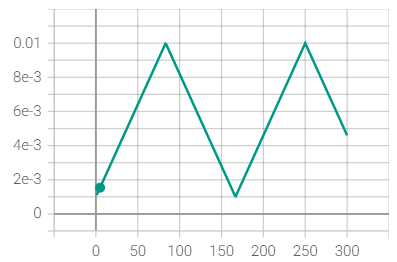
\includegraphics[scale=.9]{figures/png/cyclic_lr.png}
  \end{subfigure}
  \begin{subfigure}{0.48\textwidth}
    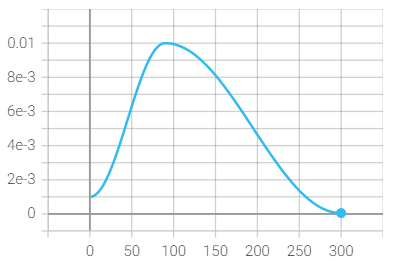
\includegraphics[scale=.9]{figures/png/one_cycle_lr.png}
  \end{subfigure}
  \caption{Learning rate schedules. The x-axis shows the epoch number, the y-axis shows the learning rate value at the given epoch. (Left) Cyclical learning rate schedule. (Right) One-cycle learning rate schedule.}
  \label{fig:learning_rate_schedules}
\end{figure}

%%%%%%%%%%%%%%%%%%%%%%%%%%%%%%%%%%%%%%%%%%%%%%%%%%%%%%%%%%%%%%%%%%%%%%%%%%%%%%%%%%%%%%%
\subsection*{Teacher Forcing, Curriculum Learning, and Scheduled Sampling}
\label{subsec:teacher_forcing}
%%%%%%%%%%%%%%%%%%%%%%%%%%%%%%%%%%%%%%%%%%%%%%%%%%%%%%%%%%%%%%%%%%%%%%%%%%%%%%%%%%%%%%%

\begin{figure}
    \centering
    \scalebox{0.6}{\input{figures/svg/teacher_forcing.pdf_tex}}
    \caption{Teacher forcing at a single time step. At train time, true previous output is part of the input used for calculating the current hidden state. At test time, the previous output of the network is used instead. After \cite{Goodfellow-et-al-2016}.}
    \label{fig:teacher_forcing}
\end{figure}

A sequence-to-sequence \ac{RNN} during processing is using its previous output $\hat{\pmb{y}}_{t-1}$, previous hidden state $\pmb{h}_{t-1}$, and current input $\pmb{x}_t$ to produce current output $\hat{\pmb{y}}_t$. If the network's outputs diverge from the target outputs $\pmb{y}_t$ introducing an error, the error will accumulate and eventually lead the network to a completely wrong part of the solution space \cite{Goodfellow-et-al-2016}. To prevent this at training time, one may supply the true target of the previous time step $\pmb{y}_{t-1}$ as the input at the current time step. Since the previous output is still incorporated in the loss function, the gradient will continue to account for it, however, the network will be more "guided" during training. At test time, the network will utilize only self-produced outputs. The act of supplying the ground truth output at time step $t-1$ as an input at time step $t$ to an \ac{RNN} is called \emph{teacher forcing} \cite{Goodfellow-et-al-2016} and is depicted in \Figure{fig:teacher_forcing}.

The guidance provided by teacher forcing is especially important in the initial phase of the training, where the network's output has still relatively high validation error. Ultimately, during test, the network should operate using only self-produced outputs (without ground truth knowledge). Therefore, the better the performance of the network during training the less guidance should be provided resulting in no guidance at test time. Decreasing the amount of ground truth output supplied throughout training is called \emph{curriculum learning}. The decrease can be fixed or random. In the latter case, for each minibatch, we "flip the coin" to determine whether teacher forcing should be used. "Flipping the coin" may be implemented as sampling from a Bernoulli distribution with parameter $\epsilon$ determining the probability of using teacher forcing. For example, at test time, we have $\epsilon=0$. This approach bears the name of \emph{scheduled sampling} \cite{Bengio2015}. Again, the $\epsilon$ parameter may be decreased with each minibatch. In this work, we only consider a linear decay of $\epsilon$.

%%%%%%%%%%%%%%%%%%%%%%%%%%%%%%%%%%%%%%%%%%%%%%%%%%%%%%%%%%%%%%%%%%%%%%%%%%%%%%%%%%%%%%%
\section*{Software for Deep Learning}
%%%%%%%%%%%%%%%%%%%%%%%%%%%%%%%%%%%%%%%%%%%%%%%%%%%%%%%%%%%%%%%%%%%%%%%%%%%%%%%%%%%%%%%

A deep learning practitioner needs to implement the designed architectures, loss functions, dataset handling, training and test procedures, etc. For this purpose, we used the PyTorch library \cite{Pytorch}. Additional functionality was provided using \cite{CoreAudioML}.

%%%%%%%%%%%%%%%%%%%%%%%%%%%%%%%%%%%%%%%%%%%%%%%%%%%%%%%%%%%%%%%%%%%%%%%%%%%%%%%%%%%%%%%
\subsection{Neural Ordinary Differential Equations}
\label{sec:neural_odes}
%%%%%%%%%%%%%%%%%%%%%%%%%%%%%%%%%%%%%%%%%%%%%%%%%%%%%%%%%%%%%%%%%%%%%%%%%%%%%%%%%%%%%%%

%TODO: Add citations
\begin{figure}
    \centering
    \begin{tikzpicture}
    \node[dspnodeopen,dsp/label=above]              (input) {$\pmb{t}, \pmb{y}_0, f(t, \pmb{y})$};
    \node[dspfilter,right=of input, minimum width=2.5cm,xshift=1cm]                                (odesolve) {\texttt{ODESolve}};
    \node[dspnodeopen,dsp/label=above,right=of odesolve,xshift=1cm]              (output) {$[\pmb{y}_0, \pmb{y}_1, \dots, \pmb{y}_{N-1}]$};

    \draw[dspconn] (input) -- (odesolve);
    \draw[dspconn] (odesolve) -- (output);
\end{tikzpicture}

    \caption{A high-level view on the ODENet architecture.}
    \label{fig:odenet_architecture}
\end{figure}

It has been observed that learning the residual instead of the function can be viewed as an Euler step of solving a differential equation. As described in \Section{subsection:forward_euler}, in the Euler method of solving \acp{ODE}, function's value at time step $t_{i+1}$ is approximated by adding the value of the derivative at time step $t_{i}$ multiplied by the time step size $t_{i+1} - t_i$ to the function's value at $t_i$. \cite{Chen2018} stated this observation explicitly and proposed to change the discrete scheme to a continuous one. In such a scheme, the network learns not the residual but the derivative of the desired function. This \emph{derivative network} is supplied to a numerical solver of choice. The loss is calculated using the solver's (not the network's) output. The backpropagation through the solver's operations can be done in constant time using the adjoint sensitivity method \cite{Chen2018}. Such generically defined architecture was named ODENet and is presented in \Figure{fig:odenet_architecture}. $t$ denotes a vector with time instances, $\pmb{y}_0$ is the initial value, such that $\pmb{y}(t[0]) = \pmb{y}_0$ (unknown function $\pmb{y}$ is assumed to be a vector-valued function for generality), and $f(t, \pmb{y})$ is the right-hand side of the \ac{ODE} we want to solve, as in \Equation{eq:general_ode}.

Long before the renaissance of deep learning, function $f(t, \pmb{y})$ supplied to the solver was a software procedure that could be evaluated for arbitrary time $t$ and function value $\pmb{y}$ (as long as it was in the domain of the function $f$). However, in the ODENet framework, $f$ \emph{is the neural network that learned to approximate the derivative function}. Ideally, the numerical solver should not be able to distinguish whether it receives a deterministic function or a neural network. However, in reality, the implementation may require an intervention into the code of the solver, for example, for \ac{GPU} optimization purposes.

The fact that $f$ may be both a function or a neural network has strong implications. First, the derivative network must be memoryless. That is caused by the fact that we may want to use an implicit solver instead of an explicit one and, thus, integrate backwards in time. If the network maintained any information from the previous calls, the changed order of evaluation could severely obscure its output and would render its use impossible for implicit solvers. Similarly, changing the step size during integration would result in incorrect network output eliminating the use of adaptive-stepsize solvers. Thus, all "state" information should be supplied explicitly as an argument in the vector $\pmb{y}$.

Second, data for ODENet training and validation can be synthesized using closed-form \acp{IVP} and numerical solvers. This helps in verifying the correctness of implementation and the possible shortcomings of the ODENet framework approach.
\cite{Karlsson2019} successfully applied ODENet to model dynamical systems, i.\ e., systems governed by \acp{ODE}. It may be regarded as a proof of concept that ODENet is, in general, applicable to dynamical systems such as analog audio effects.

Finally, the benefit of using a neural network instead of a closed-form formulation could help overcome the challenge of cases, where the closed-form derivative is limited by some assumptions (linearized, for example) or it is not known at all. If the data is governed by an \ac{ODE}, whether known or not, the ODENet should be able to learn it. This opens many exciting possibilities, on condition that the framework can actually learn the underlying dynamics.


%%%%%%%%%%%%%%%%%%%%%%%%%%%%%%%%%%%%%%%%%%%%%%%%%%%%%%%%%%%%%%%%%%%%%%%%%%%%%%%%%%%%%%%
\subsubsection{The Problem of Initialization}
%%%%%%%%%%%%%%%%%%%%%%%%%%%%%%%%%%%%%%%%%%%%%%%%%%%%%%%%%%%%%%%%%%%%%%%%%%%%%%%%%%%%%%%

As the derivative network should learn only the rate of change of the modeled function, the ODENet framework is highly susceptible to correct initialization, i.e., correct $\pmb{y}_0$ supplied as the initial value. In the extreme case, supplying a vector of zeros could lead to all-zero output. To prevent this and allow the network to be trained, one may turn to the teacher forcing approach
% TODO: as described in \Section{sec:teacher_forcing}
to ensure proper guidance during training. In the context of ODENet, teacher forcing results in supplying the ground truth initial value $\pmb{y}_0$ or all-zero vector for each minibatch according to the curriculum.

At test time, for most dynamical systems, we could also provide a meaningful initial value. After all, the goal is to predict future state from some initial state. However, in the context of \ac{VA} modeling, we can only supply an all-zero vector as the initial value because the framework should predict the whole of the output from the input. For non-zero true output, this results in increased test error.

%%%%%%%%%%%%%%%%%%%%%%%%%%%%%%%%%%%%%%%%%%%%%%%%%%%%%%%%%%%%%%%%%%%%%%%%%%%%%%%%%%%%%%%
\subsubsection{The Problem of Excitation}
%%%%%%%%%%%%%%%%%%%%%%%%%%%%%%%%%%%%%%%%%%%%%%%%%%%%%%%%%%%%%%%%%%%%%%%%%%%%%%%%%%%%%%%

In the existing applications of the ODENet framework, the derivative network was unaware of any external excitation of the system. An excitation is an important element of an \ac{ODE} that significantly influences the dynamics of the system. In the context of \ac{VA} modeling, the excitation typically consist of the input signal to the device (amplifier, distortion effect, phaser, etc.). The importance of the input signal as an excitation is visible in the diode clipper example, as discussed in \Section{subsec:diode_clipper_intro}.

How to condition the derivative network with an excitation signal? The implementation must consider the following requirements:
\begin{itemize}
  \item the excitation signal should be a part of the input to the network at each call of $f(t, \pmb{y})$,
  \item the excitation cannot be provided by the numerical solver due to the generality of their implementation,
  \item the excitation signal must be possible to evaluate for an arbitrary time given in seconds (not samples).
\end{itemize}

To facilitate incorporating the excitation signal into the framework, the following design decisions were made:
\begin{itemize}
  \item the excitation data corresponding to the current minibatch is supplied to the derivative network before calling the numerical solver for that minibatch,
  \item the values of the excitation signal are linearly interpolated using physical time values,
  \item for each minibatch, time starts at 0,
  \item the derivative network, when called with arguments $t$ and $\pmb{y}$ calculates the value of the excitation signal for that $t$ (as specified above) and concatenates with the $\pmb{y}$ vector to form the input for a single forward pass.
\end{itemize}

In the initial experiments, linear interpolation proved itself sufficient to model oscillating systems. Therefore, higher-order interpolation methods were not used in this work.

%%%%%%%%%%%%%%%%%%%%%%%%%%%%%%%%%%%%%%%%%%%%%%%%%%%%%%%%%%%%%%%%%%%%%%%%%%%%%%%%%%%%%%%
% TODO: If we actually use the "augmented state" then finish this section
%\subsubsection{The Problem of Dimensionality}
%%%%%%%%%%%%%%%%%%%%%%%%%%%%%%%%%%%%%%%%%%%%%%%%%%%%%%%%%%%%%%%%%%%%%%%%%%%%%%%%%%%%%%%

%%%%%%%%%%%%%%%%%%%%%%%%%%%%%%%%%%%%%%%%%%%%%%%%%%%%%%%%%%%%%%%%%%%%%%%%%%%%%%%%%%%%%%%
\subsection{Implementation}
%%%%%%%%%%%%%%%%%%%%%%%%%%%%%%%%%%%%%%%%%%%%%%%%%%%%%%%%%%%%%%%%%%%%%%%%%%%%%%%%%%%%%%%

The task of the ODENet is to provide an output sequence $\hat{\pmb{y}}_0, \dots, \hat{\pmb{y}}_{N-1}$ in response to an input sequence $\pmb{x} = \pmb{x}_0, \dots, \pmb{x}_{N-1}$. \Figure{fig:odenet_sequence_diagram} contains a sequence diagram of how processing is organized for a single input sequence.

% TODO: Add figure of ODENet processing.
\begin{figure}
  \centering
  \scalebox{0.9}{  \begin{sequencediagram}
    \newthread{Session}{training/test}{}
    \newinst[1]{ODENet}{:ODENet}{}
    \newinst[1]{Solver}{:ODESolver}{}
    \newinst{NN}{f:DerivativeNetwork}{}
    \newinst{interpolator}{:Interpolator}{}

    \begin{sdblock}{\shortstack{for each dataset example with input sequence $\pmb{x}$\\and target sequence $\pmb{y}_0, \dots, \pmb{y}_{N-1}$}}{}
        \postlevel

        \begin{call}{Session}{\hspace{6mm}set\_initial\_value($\pmb{y}_0$)}{ODENet}{}
        \end{call}
    
        \postlevel

        \begin{call}{Session}{forward($\pmb{x}$)}{ODENet}{$\hat{\pmb{y}}_0, \dots, \hat{\pmb{y}}_{N-1}$}
            \begin{call}{ODENet}{set\_excitation\_data($\pmb{x}$)}{NN}{}
                \begin{call}{NN}{\hspace{10mm}set\_excitation\_data($\pmb{x}$)}{interpolator}{}
                \end{call}
            \end{call}

            \postlevel

            \begin{call}{ODENet}{\hspace{1mm} integrate(f, $\pmb{y}_0$, $\pmb{t}$)}{Solver}{$\hat{\pmb{y}}_0, \dots, \hat{\pmb{y}}_{N-1}$}
                \begin{sdblock}{Solver Loop}{}
                    \begin{call}{Solver}{forward($t$, $\pmb{y}_t$)}{NN}{$\hat{\pmb{y}}'_t$}
                        \begin{call}{NN}{get\_excitation(t)}{interpolator}{$\pmb{x}_t$}                            
                        \end{call}
                    \end{call}
                \end{sdblock}

            \end{call}
        \end{call}
    \end{sdblock}
  \end{sequencediagram}
}
  \caption{Sequence diagram containing the details of ODENet processing with excitation data. }
  \label{fig:odenet_sequence_diagram}
\end{figure}

At training and test time, we loop over a dataset of examples. Examples can be processed in minibatches but it has been omitted in the figure for simplicity. First, according to the curriculum, the initial value is given to the ODENet instance. It could be the true target $\pmb{y}_0$, an all-zero vector, or possibly a different vector. Second, the ODENet is given the input sequence to process. This the excitation in the \ac{ODE} terminology. The ODENet instance passes the excitation to the derivative network, which in turn passes it to the interpolator. The interpolator instance and ODENet instance both use the same time vector $\pmb{t}$, which contains the time instances corresponding to the elements of the input sequence $\pmb{x}$, with $t[0]=0$. Third, the ODENet calls the numerical solver, passing it the network as the right-hand side of the \ac{ODE}, time vector $\pmb{t}$ that contains the time points at which to obtain the solution and the initial value $\pmb{y}_0$. Afterwards, the solver starts processing the data, which should be treated as a black-box operation, i.e., we cannot control the solver's operations. During processing, the solver will call the network, asking it to provide the value of the derivative at specific time $t$ where the solution value is $\pmb{y}_t$. The network will retrieve the excitation data from at that time instant and concatenate it with $\pmb{y}_t$ to obtain the input to the neural network that parametrizes the right-hand side of the \ac{ODE}. The result of the forward pass with this input is the estimate of the derivative of $\pmb{y}(t)$ at time $t$. The solver will call the derivative network according to its implementation; it can be at arbitrary time without any fixed time step. It must be controlled whether the derivative network is asked to provide output at time outside the time range for which it has the excitation data. If that happens, the solution can no longer be relied on. Finally, the solver returns the solution of the \ac{ODE} at requested points, which is subsequently returned as the output sequence produced in response to the input sequence $\pmb{x}$.

After obtaining the output of the ODENet, we can calculate the loss with respect to the true output $\pmb{y}_0, \dots, \pmb{y}_{N-1}$ and do a gradient step (at training time).

The input sequence can be multidimensional, i.e., one vector from the input sequence $\pmb{x}_t$ may have multiple entries, which may correspond to the input signal (e.g., guitar signal) or a control signal (e.g., \ac{LFO} signal). The vectors in the output sequence may also have multiple elements. In this work, it is assumed that the first element of each output vector is the audio output (an audible signal) whereas all other entries may correspond to a learned hidden state that is relevant for \ac{ODE} integration. Naturally, only the audible output can be used to compute the loss, unless some other state inside the analog circuit is known (as in \cite{Parker2019}, for example).
